\newcommand{\chisquare}{$\chi^2$}

\chapter{Referêncial Teórico}

\section{Esteganografia}
%-----------------------

Esteganografia, em um contexto atual, é a prática de esconder um aquivo digital dentro de outro. Estes arquivos podem ser imagens, vídeos, aúdio, ou simplesmente texto. A palavra estaganografia combina as palavras gregas \emph{steganos}, que significa ``coberto'', ou ``protegido'', e \emph{graphein}, que significa ``escrita''.

Apesar do uso moderno comumente envolver arquivos de computador, a esteganografia é uma prática antiga que tem muitos anos de história.

A esteganografia contrasta com a criptografia quanto ao aspecto da confidencialidade. A criptografia oferece um meio de comunicação seguro, onde terceiros não podem enteneer o que está sendo conversado, porém sabe que informação confidencial está sendo trocada.

O objetivo da esteganografia é modificar o arquivo portador de forma imperceptível, de maneira que nada seja revelado. Nem a presença de uma mensagem secreta e, muito menos, a mensagem secreta em si. \cite{westfeld1999attacks}

Sistemas esteganográficos geralmente funcionam processando dois parâmetros: uma mensagem secreta, e uma mensagem de cobertura. \cite{westfeld1999attacks}  % Tem uma imagem bonitinha no artigo que pode ser útil.
Alguns também precisam de uma senha para criptografar a mensagem. \cite{??}

Arquivos de múltimídia, como aúdio e vídeo, servem como exceletentes portadores. Pois contém rúido que serve de espaço para inserir uma mensagem secreta. \cite{westfeld1999attacks}

Um esteganograma deve ter as mesmas características estatísticas do aquivo original. De forma contrária, o sistema esteganográfico seria inseguro. \cite{westfeld1999attacks} Pois a presença de uma mensagem secreta seria mais facilmente detectada.

No uso moderno existem dois tipo principais de esteganografia: \emph{Least Significant Bit} (LSB) e \emph{Discrete Cosine Transform} (DCT).


\subsubsection{Least Significant Bit (LSB)}

\emph{Least Significant Bit} (LSB) (literalmente, bit menos significante) é o método mais básico de estaganografia moderna. O bit menos significativo é o que torna uma sequência de bits par ou impar. No byte \texttt{0110110\textcolor{red}{1}}, o bit menos significativo é o bit \texttt{\textcolor{red}{1}} que está na extrema esquerda.

Ao alterar o LSB o valor do byte não altera muito, se comprado a mudança a qualquer um dos outros bits. E é por isso que muitos métodos de esteganografia alteram apenas os LSBs, assim o valor de cada byte não terá uma alteração significativa. Em uma imagem, por exemplo, após aplicar o método LSB para esconder uma mensagem, os bits mais a direita terão sido alterados, mas a imagem, para o olho humano, continua a mesma. Não há mudanças perceptíveis para o olho humano.

Alterando os LSBs, a capacidade máxima que temos para esconder uma informação é de $1/8$ do tamanho do arquivo. Se uma imagem tem 152 Kilobytes, podemos esconder 19 Kilobytes (152 Kilobits) de informação.


\subsubsection{Discrete Cosine Transform (DCT)}

No formato de imagem JPEG, para cada componente de cor o formato usa \emph{Discrete Cosine Transform} (DCT) para transformar blocos de 8x8 pixels em coeficentes 64 DCTs cada. \cite{provos_hide_2003}


\section{Esteganálise}
%---------------------

A esteganálise é uma área de pesquisa que busca criar métodos para detectar quando a esteganografia foi aplicada em um item ou não.

Existem dois tipos principais de esteganálise: visuais e estatísticos. Quandos disponíveis, ataques estatísticos são superiores aos visuais, pois são menos dependentes do arquivo original e podem ser completamente automatizados, o quê permite processar vários itens em larga escala. \cite{westfeld1999attacks}

Alguns dos principais métodos de esteganálise são: Chi Square, RS Analysis, Primary Sets, Sample Pair.

\subsection{Chi Square}

O \emph{\chisquare} (Chi Square) \cite{westfeld1999attacks} é uma análise estatística dos pares de valores (PoVs) trocados durante a esteganografia LSB.
A ideia do Chi Square é comparar as distribuição de frequências téorica esperada de esteganogramas com algumas amostras da distribuição observada no item que está sendo análisado.

Sobrescrever os LSBs de uma imagem transforma alguns valores em outros valores que apenas diferem pelo LSB. Esses pares de valores são chamados de PoV. Por exemplo, \texttt{0110110\textcolor{red}{1}} forma um PoV com \texttt{0110110\textcolor{red}{0}}. Se os LSBs sobrescrescritos forem uniformemente distribuídos, as frequências dos valores de cada PoV irá se igualar. Ou seja, \texttt{0110110\textcolor{red}{1}} apareceria tantas vezes quanto \texttt{0110110\textcolor{red}{0}}. Meio-a-meio. Veja a figura \ref{fig:chi-histogram}.

\begin{figure}[ht!] % Fig. 14
\centering
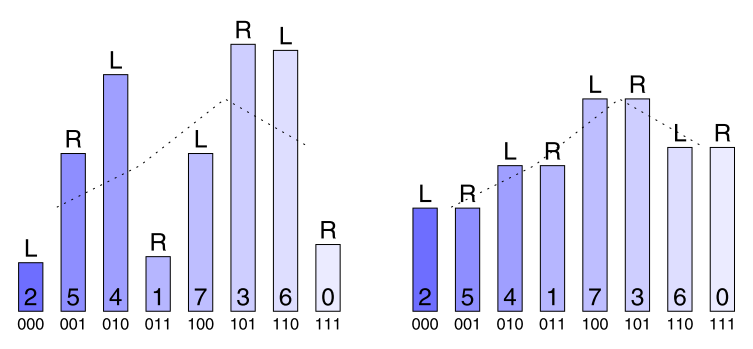
\includegraphics[width=90mm]{img/westfeld-histogram.png}
\caption{\label{fig:chi-histogram}Histograma das cores de uma imagem antes e depois de esteganografia com EzStego}
\legend{Fonte: \citeonline{westfeld1999attacks}}
\end{figure}

Um ponto crítico é como podemos obter a distribuição de frequências teoricamente esperada (i. e., a frequência de ocorrências que nós esperaríamos, após aplicarmos esteganografia)
 % A critical point is how to obtain the theoretically expected frequency distribution (i. e., the frequency of occurrence we would expect after applying stegano- graphic changes).
Essa frequência não pode ser derivada do item que está sendo análisado, porque ele pode ter sido alterado por operações esteganográficas.
 % This frequency must not be derived from our random sample, because this random sample could have been changed by steganographic op- erations.
Mas na maioria dos casos, nós não temos o arquivo original disponível para compararmos, ou para derivar a frequência esperada. No original, a frequência teoretica esperada é a média aritmética das duas frequências de um PoV.
 % But in most cases we don’t have the original to compare with or to derive the expected frequency from. In the original, the theoretically expected frequency is the arithmetic mean of the two frequencies in a PoV.
A linha tracejada na figura 14 conecta a média aritimética desses valores. Porque a esteganografia sobrescreve os LSBs, ela não muda a soma dessas duas frequências.
 % The dashed line in Fig. 14 connects these arithmetic mean values. Because the embedding function overwrites the least significant bits, it does not change the sum of these two frequencies.
O quantidade tirada dos valores ímpares é transferida para os valores pares correspondentes de cada PoV, e vice versa.
 % The count taken from the odd value frequency is transferred to the corresponding even value frequency in each PoV, and vice versa.
Como a soma é constante, a média aritmética também é a mesma para cada PoV. Tanto no arquivo original, quanto no arquivo alterado, o estanograma.
 % As the sum stays constant, the arithmetic mean is the same for a PoV in both, the original carrier medium and each corresponding steganogram.
Isso nos permite obter a distribuição de frequências teoricamente esperada através do item que está sendo analisado. Assim não precissamos do arquivo original para o ataque.
 % This fact allows us to obtain the theoretically expected frequency distribution from the random sample. So we don’t need the original carrier medium for the attack.


O gráu de similaridade entre a distribuição observada na amostra e a distribuição de frequências teoricamente esperada é a medida de probabilidade de que métodos estegaanográficos foram aplicados.
 % The degree of similarity of the observed sample distribution and the theoretically expected frequency distribution is a measure of the probability that some embedding has taken place.
Esse gráu de similaridade é determinado usando o teste Chi Square. Esse teste faz um mapeamento das observações em categorias.
 % The degree of similarity is determined using the Chi-square test (e.g., [1]). This test operates on a mapping of observations into categories. It performs the following steps:


\subsection{RS Analysis}
\cite{fridrich2001reliable}: detecta LSBs espalhados em imagens em tons de cinza ou coloridas ao inspecionar as diferenças no número de grupos regulares e singulares para os LSB e o plano LSB deslocado.

\subsection{Primary Sets}
\cite{dumitrescu2002steganalysis}: baseado em um identidade estatística relacionada a alguns conjuntos de pixels em uma imagem.

\subsection{Sample Pair}
\cite{dumitrescu2003detection}: baseado em uma máquina de estados finitos cujos estados são múltiplos conjuntos selecionados de pares de amostras chamados ``trace multisets''.


\section{Curva ROC}
%------------------


